\documentclass{article}

\pagestyle{empty}

\usepackage[margin=1in]{geometry} % Fix margins 

\usepackage{wheelchart} % Need for pie graphs
\usepackage{pgfplots} % Need for bar graphs

\usepackage{fontspec} % Enables TrueType fonts 
 	\setmainfont{Din-Pro} % Name your font

\usepackage[table]{xcolor} % Enables colors and color definition 
 	\definecolor{arcgold}{RGB}{255,184,53} 
 	\definecolor{arcgray}{RGB}{126,125,127} 
 	\definecolor{arcred}{RGB}{238,87,93} 
 	\definecolor{arcpurple}{RGB}{99,110,160} 
 	\definecolor{arcindigo}{RGB}{18,112,179} 
 	\definecolor{arcblue}{RGB}{66,173,211} 
 	\definecolor{arcteal}{RGB}{26,175,166} 
 	\definecolor{arcforest}{RGB}{103,133,57} 
 	\definecolor{arcgreen}{RGB}{152,174,62} 


\begin{document}

\begin{center}
\LARGE{\textbf{Demographic Profile: Fulton County}}\\
\end{center}

\section*{Race and Ethnicity}

\rowcolors{2}{arcgray!25}{white} % alternate gray and white rows in table
\def\arraystretch{1.25} % give some extra vspace in table

\begin{tabular}{ p{4in} r r }

& \textbf{Count} & \textbf{Percent} \\
Total Population & 1,076,561 & 100\% \\ 
Non-Hispanic White & 396,329 & 37\% \\
Non-Hispanic Black or African American & 453,703 & 42\% \\
Non-Hispanic Asian & 83,505 & 8\% \\
Non-Hispanic Other & 55,057 & 5\% \\
Hispanic or Latino, All Races & 87,967 & 8\%\\

\end{tabular}
\rowcolors{1}{}{} % Reset table row shading to default

\section*{Educational Attainment}

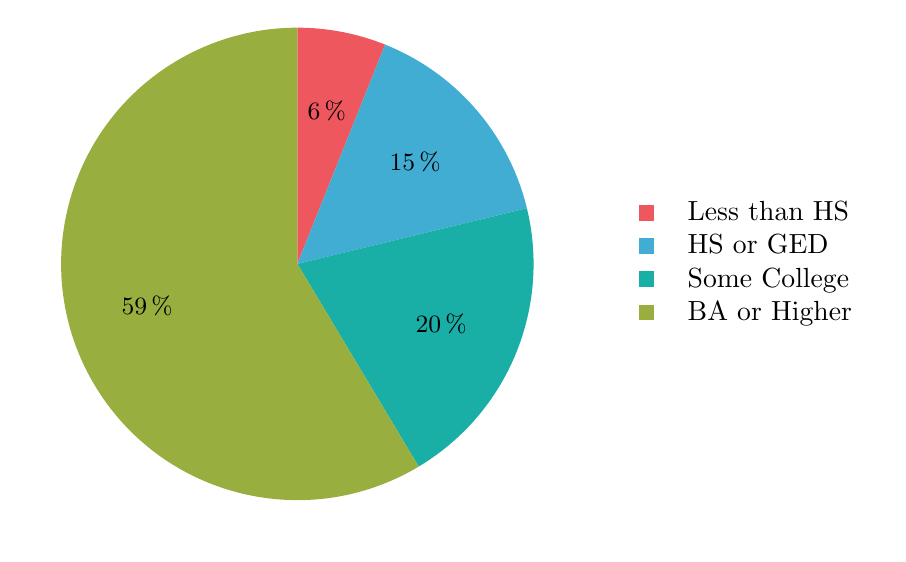
\begin{tikzpicture}
    \wheelchart[
        pie,
        radius={0}{3},
        slices style={fill=\WClistcolors, draw=none},
        WClistcolors={arcred, arcblue, arcteal, arcgreen},
        value=\WCvarA,
        % Inside Slices: Show Percentages
        wheel data=\WCperc,
        wheel data style={black, font=\small},
        % Legend: Show Labels (e.g., Less than HS)
        legend row={\tikz\fill[\WClistcolors] (0,0) rectangle (0.2,0.2); & \WCvarB},
        legend={
            \node[right] at (4,0) {
                \begin{tabular}{ll}
                    \WClegend
                \end{tabular}
            };
        },
        % Disable the default label search
        data={} 
    ]{
        6/Less than HS,
        15/HS or GED,
        20/Some College,
        58/BA or Higher
    }
\end{tikzpicture}

\section*{Housing Cost Burdened Households}

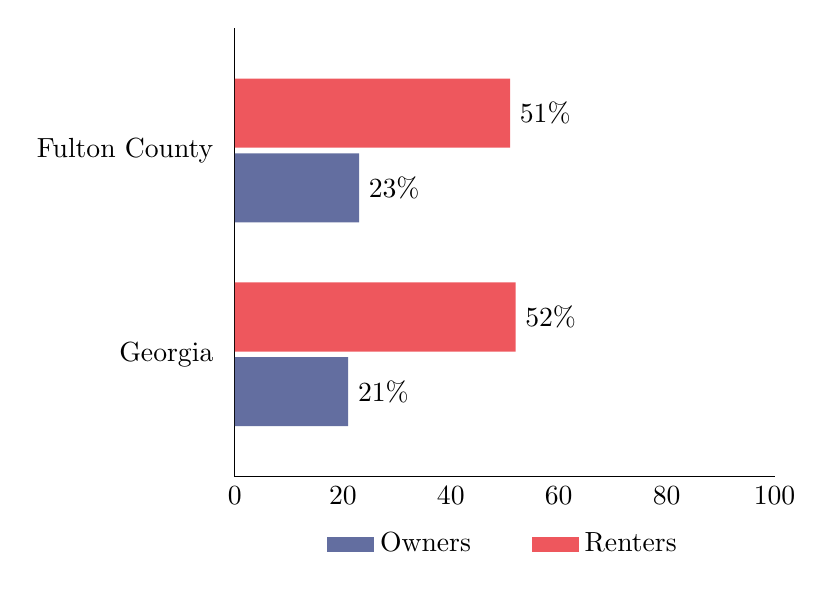
\begin{tikzpicture}
	\begin{axis}[ytick style={draw=none}, xtick style={draw=none},
	axis lines*=left,
	xbar,
	bar width=25pt, % Adjust width as needed
	enlarge x limits=0,
	enlarge y limits=0.6, % Adjust spacing as needed
	legend style={at={(0.5,-0.1)}, % Put legend below graph
	draw=none, % suppress box around legend itself
	anchor=north,legend columns=-1, % legend placement and orientation
	/tikz/every even column/.append style={column sep=20pt}
	},
		symbolic y coords={Georgia, Fulton County},
	xmin = 0,
	xmax = 100,
	ytick=data,
	nodes near coords={\pgfmathprintnumber{\pgfplotspointmeta}\%},
	nodes near coords align={horizontal},
	y tick label style={rotate=0,anchor=east},
	x tick label style={/pgf/number format/fixed, /pgf/number format/assume math mode}, 
	nodes near coords style={/pgf/number format/assume math mode}
	]
	\addplot[draw=none,fill=arcpurple] coordinates {
		(21,Georgia) (23,Fulton County)  
	};
	\addplot[draw=none,fill=arcred] coordinates {
		(52,Georgia) (51,Fulton County)  
		};

	\pgfplotsset{
		legend image code/.code={
			\draw [draw=none, #1] (0cm,-0.1cm) rectangle (0.6cm,0.1cm); % draw=none suppresses box around legend icons
		},
	}
	\legend{Owners, Renters}

	\end{axis}
\end{tikzpicture}

\end{document}


